%\documentclass{beamer}
\documentclass[handout]{beamer}

\usepackage[brazilian]{babel}
\usepackage[utf8]{inputenc}
\usepackage{graphicx}
\usepackage{fontenc}
\usepackage{color}
\usepackage{listings}
\usepackage{verbatim}
\usepackage{pxfonts}
\usepackage{graphicx}
\usetheme{Amsterdam}

\title{Desenvolvimento em comunidade}
\subtitle{A história técnica e política de um plugin do WordPress}
\author{Vinicius Massuchetto}
\date{}

\lstset{%
  breakatwhitespace,
  columns=fullflexible,
  keepspaces,
  breaklines,
  tabsize=2,
  language=PHP,
  showstringspaces=false,
  extendedchars=true,
  keywordstyle=\color{blue!80!black!100},
  identifierstyle=,
  commentstyle=\color{green!50!black!100},
  basicstyle=\footnotesize\ttfamily}

\begin{document}

\frame{\titlepage}

\section{Introdução}
\subsection{Introdução}

\begin{frame}{Download}
\begin{center}

  Código fonte da apresentação:

  \vspace{0.1cm}

  \url{https://github.com/vmassuchetto/wp-bfpui-history}

  \vspace{0.5cm}

  PDF compilado:

  \vspace{0.1cm}

  \url{http://tinyurl.com/latinoware-wp1}

\end{center}
\end{frame}

\begin{frame}{Sobre o que falaremos}
  \tableofcontents[subsectionstyle=hide]
\end{frame}

\begin{frame}{O que é o WordPress}
\begin{itemize}
  \pause \item O CMS mais utilizado no mundo
  \pause \item 10 anos de desenvolvimento
  \pause \item 18,9\% dos sites do mundo usam WordPress
  \pause \item 29,3\% das pessoas nos EUA sabem o que é WordPress
  \pause \item 2.000 temas
  \pause \item 27.000 plugins
  \pause \item 20.000 desenvolvedores pelo mundo
\end{itemize}
\end{frame}

\begin{frame}
\begin{center}
  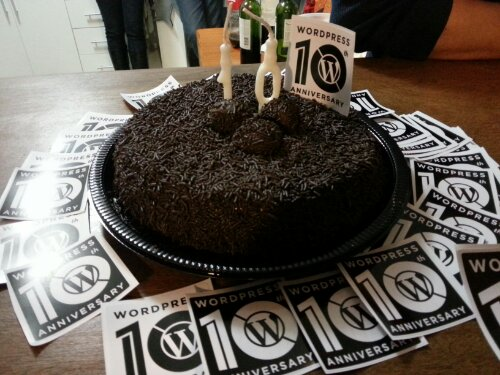
\includegraphics[width=\textwidth]{./img/wp10.jpg}
\end{center}
\end{frame}

\begin{frame}{O que são plugins do WordPress?}
\begin{itemize}
  \pause \item Rotinas que mudam o comportamento padrão do WordPress, adicionando, removendo ou modificando suas funcionalidades
  \pause \item Qualquer coisa que está no diretório \texttt{wp-content/plugins} e tem este cabeçalho:
\end{itemize}
\end{frame}

\begin{frame}
  \lstinputlisting{./code/header.php}
\end{frame}

\begin{frame}
\begin{center}
  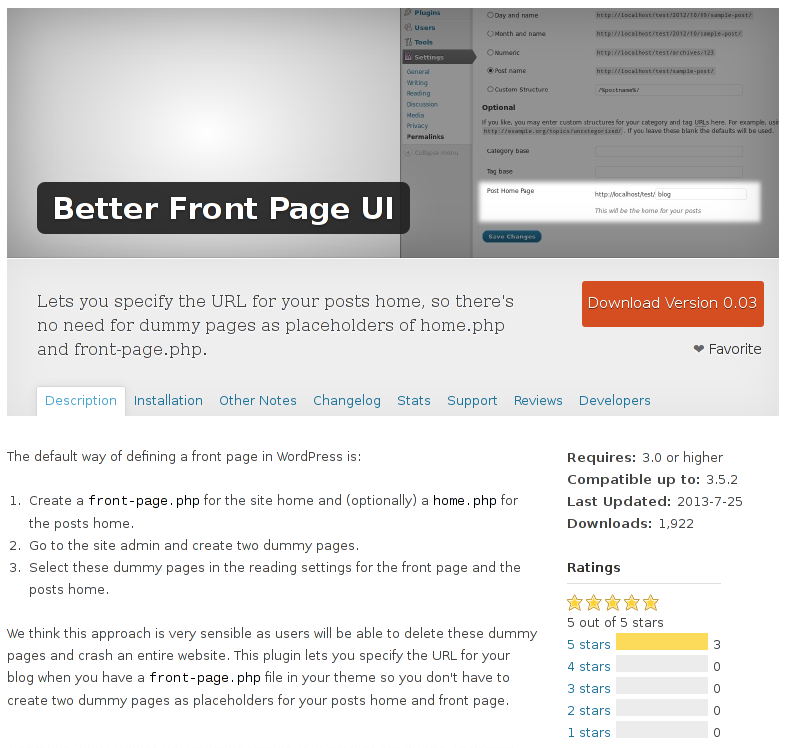
\includegraphics[width=\textwidth]{./img/plugin-screenshot.png}
\end{center}
\end{frame}

\begin{frame}{Por que esse plugin?}
\begin{itemize}
  \pause \item O propósito é reduzido, porém amplo
  \pause \item A implementação é simples, porém complexa
\end{itemize}
\end{frame}

\begin{frame}{Falando em números: aspecto técnico}
\begin{itemize}
  \pause \item 163 linhas
  \pause \item 9 commits realizados
  \pause \item 3 versões
  \pause \item 2 desenvolvedores
  \pause \item 1 plugin
\end{itemize}
\end{frame}

\begin{frame}{Falando em números: aspecto político}
\begin{itemize}
  \pause \item 189 mensagens trocadas no Trac e na wp-hackers
  \pause \item 20 core patches propostos
  \pause \item 10 propostas de usabilidade
  \pause \item 1 novo campo no admin
\end{itemize}
\end{frame}

\begin{frame}
\begin{center}
  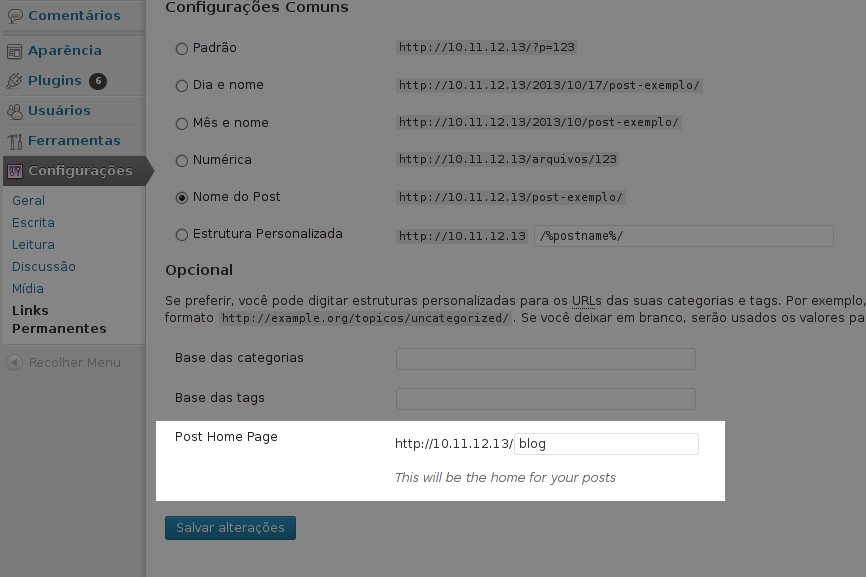
\includegraphics[width=0.9\textwidth]{./img/option-plugin-field.png}
\end{center}
\end{frame}

\section{Problema}
\subsection{Problema}

\begin{frame}{Causas dos problemas}
\begin{itemize}
  \pause \item Regra do confusa no controlador para a escolha de templates
  \pause \item Terminologia conflituosa
  \pause \item Alta sensibilidade às ações do usuário
\end{itemize}
\end{frame}

\begin{frame}{Consequências dos problemas}
\begin{itemize}
  \pause \item Temas construídos invariavelmente de forma errada
  \pause \item Confusão evitável na documentação
  \pause \item Perda de visões de conteúdo
  \pause \item Visões de conteúdo não desejadas
  \pause \item Sites fora do ar
\end{itemize}
\end{frame}

\begin{frame}
\begin{center}
  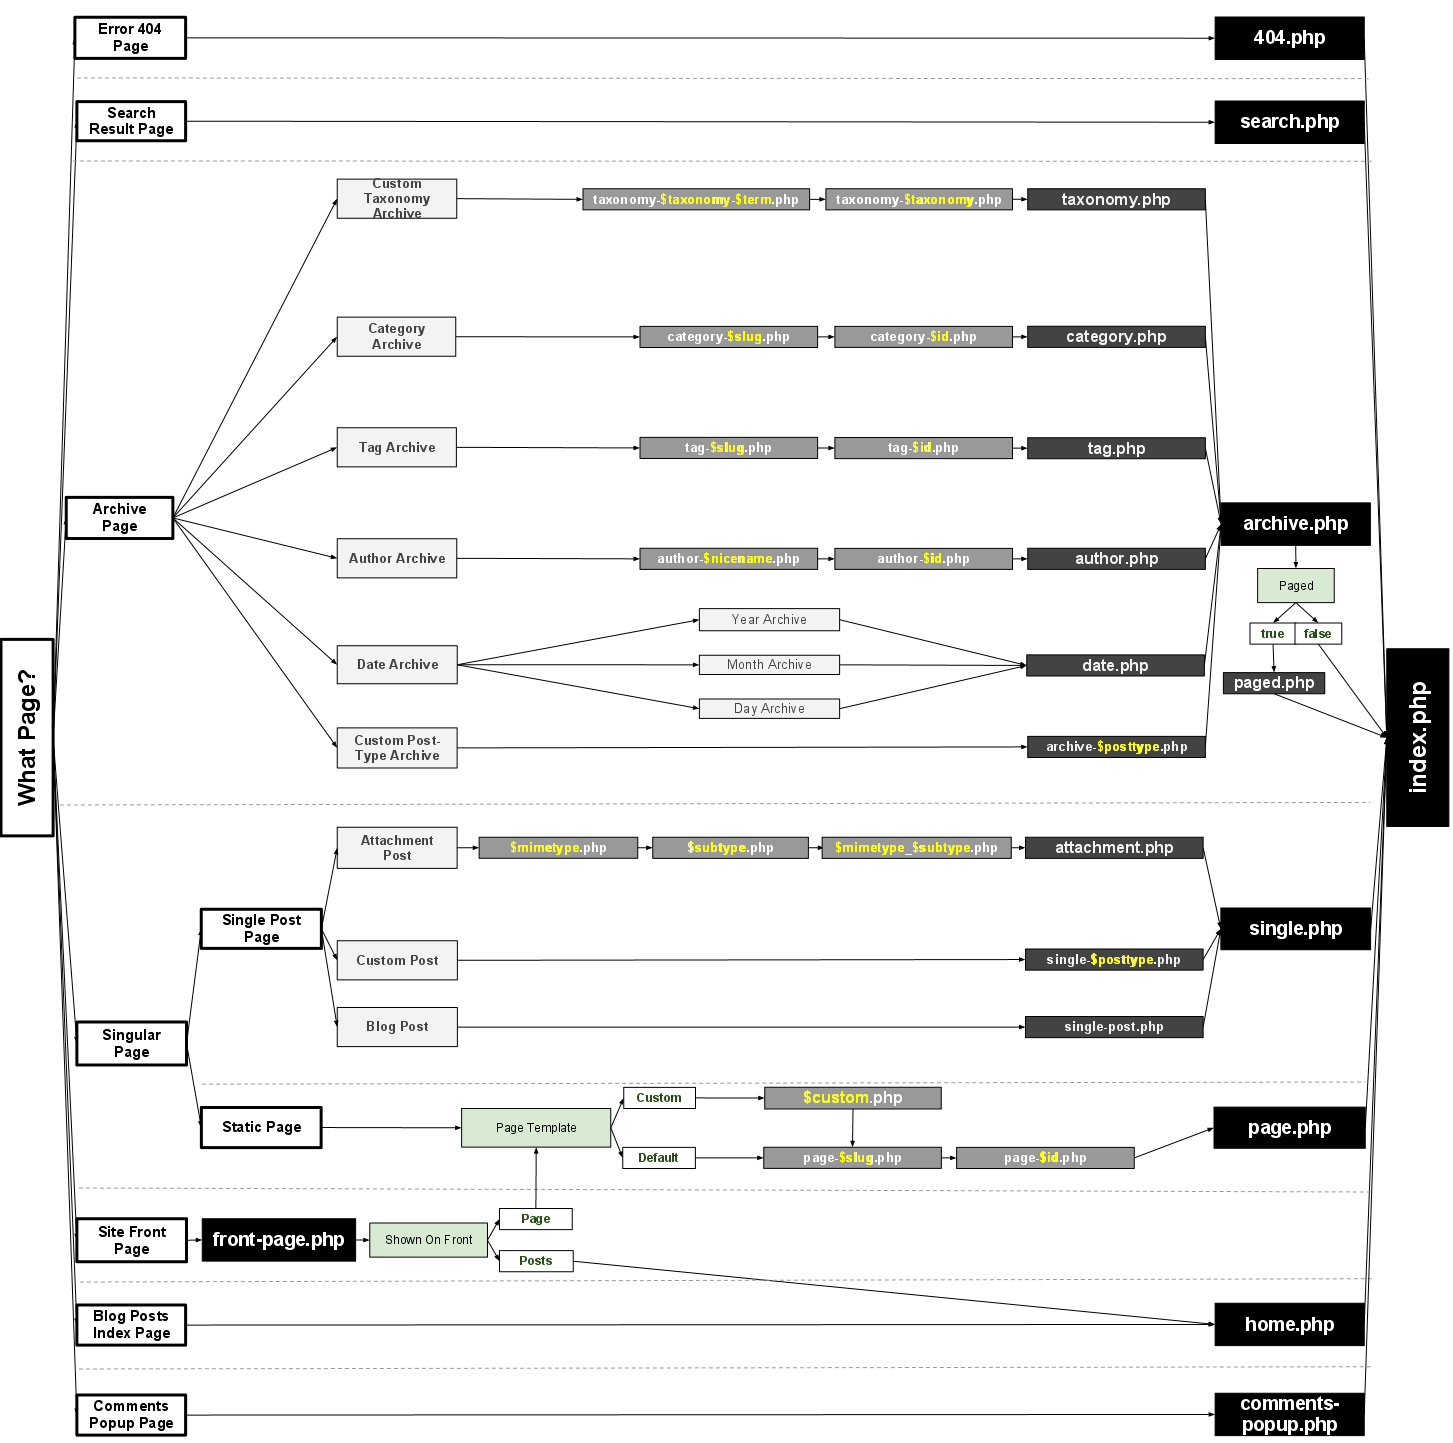
\includegraphics[height=0.9\textheight]{./img/template-hierarchy.png}
\end{center}
\end{frame}

\begin{frame}{Exemplos de hierarquia de template: datas}
\begin{itemize}
  \pause \item \texttt{http://site/2010} \\
    \pause \texttt{http://site/2010/09} \\
    \pause \texttt{http://site/2010/09/22}
  \pause \item $\rightarrow$ \texttt{date.php} \\
    \pause $\rightarrow$ \texttt{archive.php} \\
    \pause $\rightarrow$ \texttt{index.php} $\star$
\end{itemize}
\end{frame}

\begin{frame}{Exemplos de hierarquia de template: post do tipo livro}
\begin{itemize}
  \pause \item \texttt{http://site/qualquer-post-do-tipo-livro/}
  \pause \item $\rightarrow$ \texttt{single-livros.php} \\
    \pause $\rightarrow$ \texttt{single.php} \\
    \pause $\rightarrow$ \texttt{index.php} $\star$
\end{itemize}
\end{frame}

\begin{frame}{Exemplos de hierarquia de template: categoria}
\begin{itemize}
  \pause \item \texttt{http://site/category/qualquer-categoria}
  \pause \item $\rightarrow$ \texttt{category-minha-categoria.php} \\
    \pause $\rightarrow$ \texttt{category-22.php} \\
    \pause $\rightarrow$ \texttt{category.php} \\
    \pause $\rightarrow$ \texttt{archive.php} \\
    \pause $\rightarrow$ \texttt{index.php} $\star$
\end{itemize}
\end{frame}

\begin{frame}{Exemplos de hierarquia de template: lista dos livros de história}
\begin{itemize}
  \pause \item \texttt{http://site/livros/historia}
  \pause \item $\rightarrow$ \texttt{taxonomy-livros-historia.php} \\
    \pause $\rightarrow$ \texttt{taxonomy-livros.php} \\
    \pause $\rightarrow$ \texttt{taxonomy.php} \\
    \pause $\rightarrow$ \texttt{archive.php} \\
    \pause $\rightarrow$ \texttt{index.php} $\star$
\end{itemize}
\end{frame}

\begin{frame}{Exemplos de hierarquia de template: página inicial}
\begin{itemize}
  \pause \item \texttt{http://site/}
  \pause \item $\rightarrow$ \texttt{p*-problema.php} $\star$
\end{itemize}
\end{frame}

\begin{frame}
\begin{center}
  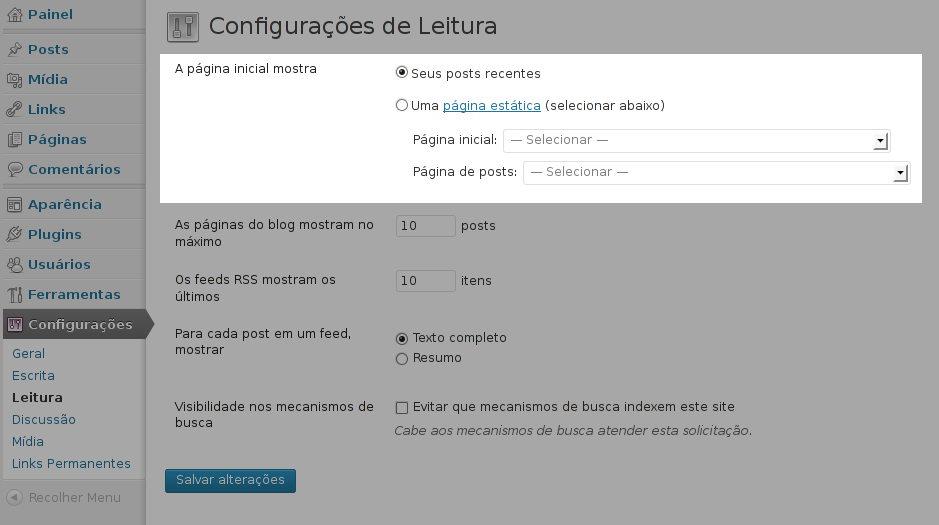
\includegraphics[width=0.9\textwidth]{./img/option-show-on-front.png}
\end{center}
\end{frame}

\begin{frame}{O problema das \emph{dummy pages}}
\begin{itemize}
  \pause \item{\texttt{get\_option( 'show\_on\_front' )}} \\
    \pause \texttt{== 'posts'} $\rightarrow$ lista de posts na página inicial,
      como usual \\
    \pause \texttt{== 'page'} $\rightarrow$ condiciona a seguinte escolha de
      templates:
\end{itemize}
\end{frame}

\begin{frame}{O problema das \emph{dummy pages}}
\begin{itemize}
  \pause \item \texttt{int( get\_option( 'page\_on\_front' ) )} \\
    \pause $\rightarrow$ \texttt{front-page.php} \\
    \pause $\rightarrow$ \texttt{page-minha-pagina.php} \\
    \pause $\rightarrow$ \texttt{page-22.php} \\
    \pause $\rightarrow$ \texttt{page.php} \\
    \pause $\rightarrow$ \texttt{index.php} $\star$
  \pause \item \texttt{int( get\_option( 'page\_for\_posts' ) )} \\
    \pause $\rightarrow$ \texttt{home.php} \\
    \pause $\rightarrow$ \texttt{index.php} $\star$
\end{itemize}
\end{frame}

\begin{frame}
\begin{center}
  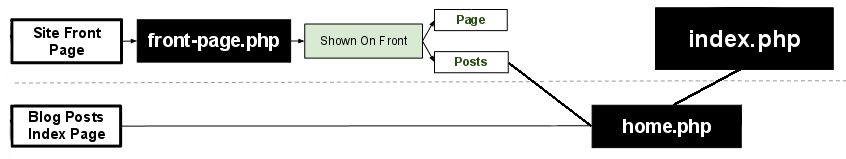
\includegraphics[width=\textwidth]{./img/template-hierarchy-front.png}
\end{center}
\end{frame}

\begin{frame}{Exemplos de hierarquia de template: página inicial}
\begin{itemize}
  \pause \item \texttt{http://site/}
  \pause \item $\rightarrow$ (\texttt{p*-problema.php})
  \pause \item $\rightarrow$ \texttt{front-page.php}
  \pause \item $\rightarrow$ \texttt{home.php}
  \pause \item $\rightarrow$ \texttt{index.php} $\star$ (?)
  \pause \item \ldots e vai ficar sem a listagem de posts principal
\end{itemize}
\end{frame}

\begin{frame}{Problema}
\begin{itemize}
  \pause \item Criação origatória das \emph{dummy pages} para ter a completude
    de funcionalidades para os templates
  \pause \item Solução sensível à interferência do usuário
\end{itemize}
\end{frame}

\section{Solução diplomática}
\subsection{Solução diplomática}

\begin{frame}{Na wp-hackers}
\begin{center}
  \emph{``Em um desenvolvimento encomendado, o desenvolvedor nada mais é do que
  um agente do usuário, que é o cliente. Não existe razão para o desenvolvedor,
  que desenvolve, instala, e configura o Tema, não possa também configurar as
  opções de leitura para que o site exiba o conteúdo adequadamente.

  \vspace{0.3cm}

  De qualquer forma, o caso de uso que você descreve não é aquele compartilhado
  pela grande maioria dos usuários do WordPress, e a habilidade do tema em
  editar o que vai aparecer na capa do site seria danoso para esta grande
  maioria.''}
\end{center}

-- Chip Bennett

\end{frame}

\begin{frame}{Na wp-hackers}
\begin{center}
  \emph{``Se você não quer o seu cliente mudando as opções do site, então não o
  cadastre como um admin.

  \vspace{0.3cm}

  Mas eu concordo com alguns comentários que pode ser confuso ver duas páginas
  que não servem pra nada no admin. Uma modificação útil seria um aviso no topo
  destas páginas avisando que elas servem para o que o Tema exiba as
  informações corretas.''}
\end{center}

-- Bill Erickson

\end{frame}

\begin{frame}{Na wp-hackers}
\begin{center}
  \emph{``Eu acho que vocês não estão entendendo a questão do Chip sobre como
  os temas não devem ditar a estrutura do site para a grande maioria dos
  usuários. É sobre quem controla o site, e não o tipo de site que é feito.}
\end{center}

-- Justin Tadlock

\end{frame}

\begin{frame}
\begin{center}
  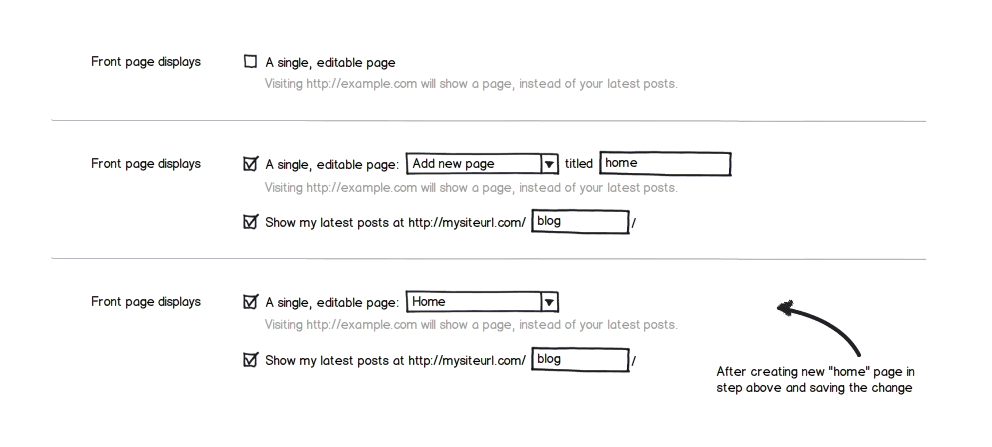
\includegraphics[width=\textwidth]{./img/proposal-dave-martin.png}
\end{center}

-- Dave Martin

\end{frame}

\begin{frame}
\begin{center}
  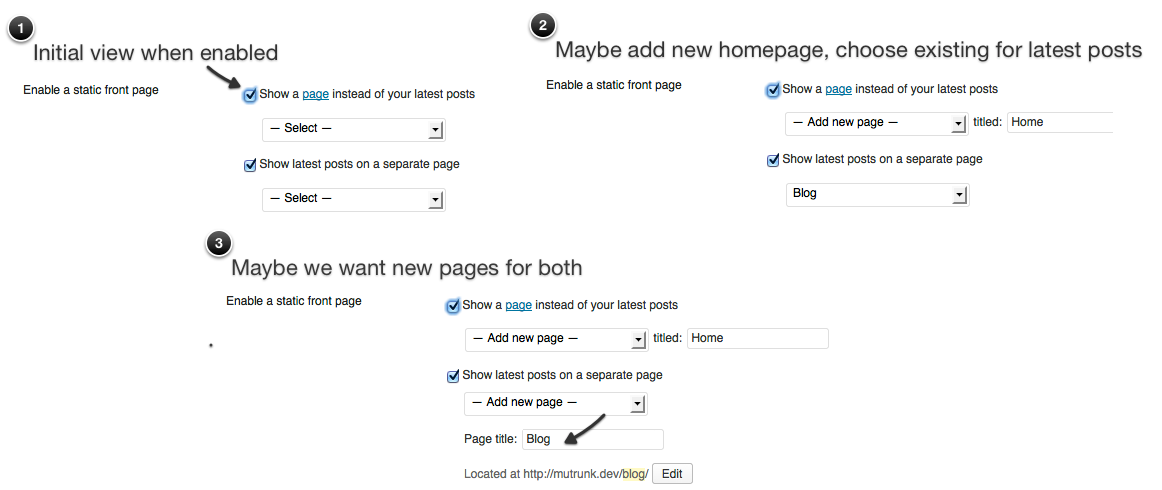
\includegraphics[height=0.8\textheight]{./img/proposal-drew-jaynes.png}
\end{center}

-- Drew Jaynes

\end{frame}

\begin{frame}{No Trac}
\begin{itemize}
  \pause \item Jan 2011: Questão aberta por Mark Jaquith sobre a usabilidade
    desta seção do admin
  \pause \item Out 2012: Funcionalidade considerada crítica e de alta
    prioridade
  \pause \item Nov 2012: Complicações de usabilidade e urgência de liberação de
    versões fazem as propostas de patches serem agendadas para um release
    indefinido. ``Faço isso com peso no coração.'' -- Andrew Nacin, ao tirar a
    funcionalidade da milestone
  \pause \item Jan 2013: Última resposta sobre esta questão
\end{itemize}
\end{frame}

\section{Solução prática}
\subsection{Solução prática}

\begin{frame}
  \pause \lstinputlisting[firstline=1,lastline=1]{./code/base-structure.php}
  \pause \lstinputlisting[firstline=2,lastline=11]{./code/base-structure.php}
  \pause \lstinputlisting[firstline=12,lastline=15]{./code/base-structure.php}
\end{frame}

\begin{frame}
  \pause \lstinputlisting[firstline=1,lastline=1]{./code/admin-field.php}
  \pause \lstinputlisting[firstline=2,lastline=4]{./code/admin-field.php}
  \pause \lstinputlisting[firstline=5,lastline=7]{./code/admin-field.php}
  \pause \lstinputlisting[firstline=8,lastline=12]{./code/admin-field.php}
\end{frame}

\begin{frame}
  \pause \lstinputlisting[firstline=1,lastline=1]{./code/rewrite-rule.php}
  \pause \lstinputlisting[firstline=2,lastline=2]{./code/rewrite-rule.php}
  \pause \lstinputlisting[firstline=3,lastline=10]{./code/rewrite-rule.php}
  \pause \lstinputlisting[firstline=11,lastline=11]{./code/rewrite-rule.php}
  \pause \lstinputlisting[firstline=12,lastline=15]{./code/rewrite-rule.php}
\end{frame}

\begin{frame}
  \pause \lstinputlisting[firstline=1,lastline=1]{./code/remove-show-on-front.php}
  \pause \lstinputlisting[firstline=2,lastline=2]{./code/remove-show-on-front.php}
  \pause \lstinputlisting[firstline=3,lastline=5]{./code/remove-show-on-front.php}
\end{frame}

\begin{frame}
  \pause \lstinputlisting[firstline=1,lastline=1]{./code/cleanup.php}
  \pause \lstinputlisting[firstline=2,lastline=3]{./code/cleanup.php}
  \pause \lstinputlisting[firstline=4,lastline=5]{./code/cleanup.php}
  \pause \lstinputlisting[firstline=6,lastline=10]{./code/cleanup.php}
\end{frame}

\begin{frame}
  \pause \lstinputlisting[firstline=1,lastline=1]{./code/blog-url.php}
  \pause \lstinputlisting[firstline=2,lastline=6]{./code/blog-url.php}
  \pause \lstinputlisting[firstline=7,lastline=10]{./code/blog-url.php}
\end{frame}

\section{Considerações finais}
\subsection{Considerações finais}

\begin{frame}{Quebrando o sono}
\begin{itemize}
  \pause \item Por que eu preciso reiniciar as regras de URL ao
    ativar e desativar o plugin, mas não ao salvar a opção no formulário?
  \pause \item Se a opção tivesse que ser colocada fora do
    \texttt{options-permalink.php}, precisaríamos salvá-la?
\end{itemize}
\end{frame}

\begin{frame}{Considerações finais}
\begin{itemize}
  \pause \item Antes de fazer um plugin que interfira no funcionamento
    estrutural do WordPress, verifique as discussões na comunidade e no Trac.
  \pause \item Uma funcionalidade simples pode vir a ser elaborada do ponto de
    vista técnico, e inviável do ponto de vista político
\end{itemize}
\end{frame}

\begin{frame}
\begin{center}

  
\includegraphics[height=0.6\textheight]{./img/thank-you.jpg}

  Plugin Better Front Page UI

  \texttt{http://wordpress.org/plugins/better-front-page-ui/}

\end{center}
\end{frame}

\end{document}
